\documentclass[aspectratio=169]{beamer}

% Theme & Basic Setup
\usetheme{Madrid}
\usefonttheme{serif}
\usepackage[T1]{fontenc}
\renewcommand{\ttdefault}{pcr}          % Courier for \texttt (code snippets)
\usepackage[scaled=1.12]{Alegreya}   % body font: Alegreya (needs TeX Live fonts-extra / MacTeX full)
\usepackage{tikz}
\usepackage{algorithm}
\usepackage{algorithmicx}
\usepackage{algpseudocode}
\usepackage{booktabs}
\usepackage{multirow}
\usepackage{colortbl}
\usepackage{graphicx}
\usepackage{amsmath}
\usepackage{hyperref}
\usepackage[normalem]{ulem}   % needed for \uline in the slide titles
\usetikzlibrary{positioning, arrows.meta, shapes, shapes.geometric, arrows}
\graphicspath{{images/}{../images/}}   % all pictures live in the images folder (../images when compiling from inside Lectures)

% Colors
\definecolor{darkblue}{RGB}{25,25,112}
\definecolor{midblue}{RGB}{65,105,225}
\definecolor{lightblue}{RGB}{173,216,230}
\definecolor{titleblue}{RGB}{30,60,180}
\definecolor{headerblue}{RGB}{20,40,120}
\definecolor{tealcustom}{RGB}{0,128,128}
\definecolor{redcustom}{RGB}{180,30,30}
\definecolor{graytext}{RGB}{120,120,120}
\definecolor{greencustom}{RGB}{34,139,34}
\definecolor{orangecustom}{RGB}{210,105,30}
\definecolor{purplecustom}{RGB}{102,51,153}
\definecolor{accentred}{RGB}{200,60,60}

% Custom Footer
\setbeamertemplate{footline}{
  \hbox{%
    \begin{beamercolorbox}[wd=.3\paperwidth,ht=2.5ex,dp=1ex,center]{author in head/foot}%
      \insertshortauthor~(\insertshortinstitute)
    \end{beamercolorbox}%
    \begin{beamercolorbox}[wd=.40\paperwidth,ht=2.5ex,dp=1ex,center]{title in head/foot}%
      \insertshorttitle
    \end{beamercolorbox}%
    \begin{beamercolorbox}[wd=.3\paperwidth,ht=2.5ex,dp=1ex,right]{date in head/foot}%
      \insertshortdate \hspace{3ex} \insertframenumber/\inserttotalframenumber \hspace{2ex}
    \end{beamercolorbox}%
  }
}

\setbeamercolor{author in head/foot}{bg=darkblue, fg=white}
\setbeamercolor{title in head/foot}{bg=midblue, fg=white}
\setbeamercolor{date in head/foot}{bg=lightblue, fg=black}

% Bullets
\setbeamertemplate{itemize item}{\color{midblue}\tiny$\blacksquare$}
\setbeamertemplate{itemize subitem}{\color{tealcustom}\scriptsize$\square$}
\setbeamertemplate{section in toc}{
  \leavevmode\leftskip=0.4em
  \tikz[baseline=(char.base)]\node[shape=circle,draw=midblue,fill=lightblue!35,inner sep=1.3pt](char){\textcolor{darkblue}{\scriptsize\textbf{\inserttocsectionnumber}}};
  \hspace{0.6em}\textcolor{titleblue}{\textbf{\inserttocsection}}\par
}
\setbeamertemplate{subsection in toc}{
  \leavevmode\leftskip=2.2em
  \textcolor{tealcustom}{\scriptsize$\blacktriangleright$}\hspace{0.5em}\textcolor{tealcustom}{\inserttocsubsection}\par
}

% Layout for the \frame[t]{\small ...} slide format
\setbeamertemplate{navigation symbols}{}
\hyphenpenalty=10000 \exhyphenpenalty=10000   % never hyphenate words on slides
\setbeamersize{text margin left=0.6cm, text margin right=0.6cm}

% Small text shortcuts (colors only)
\newcommand{\pu}[1]{\textcolor{purplecustom}{#1}}
\newcommand{\bl}[1]{\textcolor{blue}{#1}}

% Card styles (defined here because of the # parameter)
\tikzset{
  tipcard/.style={draw=#1, fill=#1!6, rounded corners=4pt, thick, minimum width=4.35cm, minimum height=1.75cm, text width=4.0cm, align=left, inner sep=5pt},
  widecard/.style={draw=#1, fill=#1!6, rounded corners=4pt, thick, minimum width=6.9cm, minimum height=1.85cm, text width=6.5cm, align=left, inner sep=6pt}
}

% Round photo of the instructor (me.jpg)
\newcommand{\mepic}{%
\begin{tikzpicture}
  \begin{scope}
    \clip (0,0) circle (1.6cm);
    \fill[white] (-2,-2) rectangle (2,2);
    \node at (0,-0.25) {\includegraphics[width=4.92cm]{me.jpg}};
  \end{scope}
  \draw[midblue, line width=2pt] (0,0) circle (1.6cm);
\end{tikzpicture}}

% Excel colors
\definecolor{excelgreen}{RGB}{33,115,70}
\definecolor{gridgray}{RGB}{210,210,210}
% All screenshots live in figures-lec2.pdf, one per page:
%  1 raw data     2 window      3 last row     4 frozen       5 freeze menu   6 before      7 after       8 format cells
%  9 formula bar 10 CF menu    11 CF dialog   12 CF result   13 sort dialog  14 sorted     15 filter menu 16 filtered

% Screenshot with a thin frame
\setlength{\fboxsep}{0pt}
\newcommand{\fig}{figures-lec2.pdf}
\newcommand{\shoth}[2]{\fcolorbox{gridgray}{white}{\includegraphics[height=#1,page=#2]{\fig}}}
\newcommand{\shot}[2]{\fcolorbox{gridgray}{white}{\includegraphics[width=\dimexpr#1-2\fboxrule\relax,page=#2]{\fig}}}

% Numbered steps (circles) and a small key-cap look for shortcuts
\setbeamertemplate{enumerate items}[circle]
\newcommand{\key}[1]{\texttt{#1}}
\newcommand{\steps}{\setlength{\itemsep}{0.55em}\footnotesize}

% Title Info
\title[ICT 101: Lecture 2]{Applications of ICT (ICT 101)\\Lecture 2: Working with Real Data in Excel}
\author[Abdul Basit]{Mr. Abdul Basit\\\small Lab Instructor}
\institute[NIT]{School of Data Science and Information Technology\\NIT}
\date[Fall 2026]{Fall 2026}

\begin{document}

% ============================================================
%  Title
% ============================================================
\begin{frame}
  \titlepage
  \begin{center}
        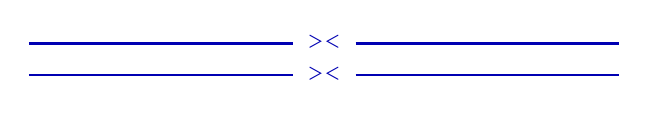
\begin{tikzpicture}
        \draw[thick, blue!70!black] (-3.75,0) -- (-0.4,0);
        \node[text=blue!70!black] at (0,0) {\texttt{><}};
        \draw[thick, blue!70!black] (0.4,0) -- (3.75,0);
        \draw[thick, blue!70!black] (-3.75,-0.4) -- (-0.4,-0.4);
        \node[text=blue!70!black] at (0,-0.4) {\texttt{><}};
        \draw[thick, blue!70!black] (0.4,-0.4) -- (3.75,-0.4);
        \end{tikzpicture} \\
  \textcolor{teal}{\small Excel Lesson 1: Navigating, Formatting, Sorting \& Filtering}
  \end{center}
\end{frame}

% ============================================================
%  Agenda
% ============================================================
\frame[t]{\small
\vskip.0in
{\large{\color{blue}{\uline{Today's Agenda\hfill}}}}
\vskip.12in

\tableofcontents
}

% %%%%%%%%%%%%%%%%%%%%%%%%%%%%%%%%%%%%%%%%%%%%%%%%%%%%%%%%%%%%
\section{Start Here}
% %%%%%%%%%%%%%%%%%%%%%%%%%%%%%%%%%%%%%%%%%%%%%%%%%%%%%%%%%%%%

% ============================================================
%  Meet the data
% ============================================================
\frame[t]{\small
\vskip.0in
{\large{\color{blue}{\uline{Meet Today's Data: 1,000 Orders\hfill}}}}
\vskip.1in

\begin{columns}[T]
\column{.62\textwidth}
\shot{\linewidth}{1}

\column{.36\textwidth}
{\color{purplecustom}\textbf{Lab2-dataset.xlsx}}

\vskip.04in
\begin{itemize}
\footnotesize
\setlength{\itemsep}{0.2em}
\item \textbf{1,000} online orders, July 2025 to June 2026
\item \textbf{14} columns: city, product, price, payment, status, rating\ldots
\item One \textbf{row} is one order, one \textbf{column} is one detail
\end{itemize}

\vskip.06in
\begin{block}{The manager asks}
\footnotesize
How many Karachi electronics orders?\\
Which item was the most expensive?\\
How many orders came back?

\vskip.04in
{\color{purplecustom}Scrolling will not answer these. By 11:35, you will.}
\end{block}
\end{columns}
}

% ============================================================
%  Open and save
% ============================================================
\frame[t]{\small
\vskip.0in
{\large{\color{blue}{\uline{Step by Step: Open the File and Save Your Own Copy\hfill}}}}
\vskip.12in

\begin{columns}[T]
\column{.56\textwidth}
\begin{enumerate}
\steps
\item Download \textbf{Lab2-dataset.xlsx} from Canvas and open it in Excel
\item Click \textbf{File} $\rightarrow$ \textbf{Save As}
\item In the name box type \texttt{RollNo\_Lab2} and use your own roll number, for example \texttt{23-NIT-0145\_Lab2}
\item Make sure the type says \textbf{Excel Workbook (.xlsx)}, then click \textbf{Save}
\item At the bottom of the window, click the \textbf{+} next to the sheet tab \texttt{Orders}
\item Double-click the new tab, type \texttt{Answers} and press \key{Enter}
\end{enumerate}

\column{.42\textwidth}
\begin{block}{Why we do this first}
\footnotesize
The original file stays untouched, so you can always download it again.

\vskip.05in
Your answers go on the \textbf{Answers} sheet: question number in column A, your answer in column B.

\vskip.05in
Press \key{Ctrl + S} after every task.
\end{block}

\vskip.1in
\begin{center}
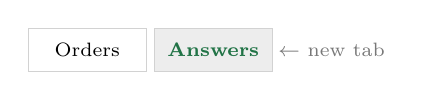
\begin{tikzpicture}[every node/.style={font=\scriptsize}]
 \node[draw=gridgray, fill=white, minimum width=1.5cm, minimum height=0.55cm] (a) at (0,0) {Orders};
 \node[draw=gridgray, fill=gridgray!40, minimum width=1.5cm, minimum height=0.55cm, text=excelgreen] (b) at (1.6,0) {\textbf{Answers}};
 \node[text=graytext] at (3.1,0) {$\leftarrow$ new tab};
\end{tikzpicture}
\end{center}
\end{columns}
}

% %%%%%%%%%%%%%%%%%%%%%%%%%%%%%%%%%%%%%%%%%%%%%%%%%%%%%%%%%%%%
\section{Getting Around}
% %%%%%%%%%%%%%%%%%%%%%%%%%%%%%%%%%%%%%%%%%%%%%%%%%%%%%%%%%%%%

% ============================================================
%  Excel window with labels
% ============================================================
\frame[t]{\small
\vskip.0in
{\large{\color{blue}{\uline{The Excel Window: Seven Parts You Will Use Today\hfill}}}}
\vskip.06in

\begin{columns}[T]
\column{.6\textwidth}
\begin{tikzpicture}
 \node[anchor=south west, inner sep=0] (img) at (0,0) {\shot{.97\linewidth}{2}};
 \begin{scope}[x={(img.south east)}, y={(img.north west)}, lab/.style={circle, fill=accentred, text=white, font=\scriptsize\bfseries, inner sep=1.2pt}]
  \node[lab] at (0.47,0.90) {1};
  \node[lab] at (0.075,0.832) {2};
  \node[lab] at (0.26,0.832) {3};
  \node[lab] at (0.355,0.80) {4};
  \node[lab] at (0.018,0.50) {5};
  \node[lab] at (0.11,0.047) {6};
  \node[lab] at (0.62,0.016) {7};
 \end{scope}
\end{tikzpicture}

\column{.38\textwidth}
\footnotesize
\renewcommand{\arraystretch}{1.35}
\begin{tabular}{@{}cp{4.7cm}@{}}
\textcolor{accentred}{\textbf{1}} & \textbf{Ribbon:} all commands, sorted into tabs (Home, Data, View)\\
\textcolor{accentred}{\textbf{2}} & \textbf{Name Box:} shows which cell is selected, and lets you jump to any cell\\
\textcolor{accentred}{\textbf{3}} & \textbf{Formula Bar:} shows what is really stored in the cell\\
\textcolor{accentred}{\textbf{4}} & \textbf{Column letters:} A, B, C\ldots\\
\textcolor{accentred}{\textbf{5}} & \textbf{Row numbers:} 1, 2, 3\ldots\\
\textcolor{accentred}{\textbf{6}} & \textbf{Sheet tab:} one tab per sheet\\
\textcolor{accentred}{\textbf{7}} & \textbf{Status bar:} count, sum and average of what you select\\
\end{tabular}
\end{columns}

\vskip.04in
{\footnotesize A cell's name is its column letter plus its row number. The cell in column \textbf{G}, row \textbf{500}, is \textbf{G500}.}
}

% ============================================================
%  Navigation steps
% ============================================================
\frame[t]{\small
\vskip.0in
{\large{\color{blue}{\uline{Step by Step: Jump Around 1,000 Rows with the Keyboard\hfill}}}}
\vskip.1in

\begin{columns}[T]
\column{.54\textwidth}
\begin{enumerate}
\steps
\item Click cell \textbf{A1}
\item Press \key{Ctrl + Down Arrow}. You land on the \textbf{last order}. Look at the row number on the left
\item Press \key{Ctrl + Right Arrow}. You land on the \textbf{last column}. Look at the column letter on top
\item Press \key{Ctrl + Home}. You are back at \textbf{A1}
\item Press \key{Ctrl + Left Arrow}, then \key{Ctrl + Up Arrow} to see how the same trick works in the other directions
\end{enumerate}

\vskip.08in
\begin{block}{The rule behind it}
\footnotesize
\key{Ctrl} + an arrow key runs to the \textbf{edge of the filled cells} in that direction. It stops where the data stops.
\end{block}

\column{.44\textwidth}
\shot{\linewidth}{3}

\vskip.04in
{\scriptsize\color{graytext}After step 2: the Name Box and the row numbers show where you landed. The data ends at row 1001.}

\vskip.08in
\renewcommand{\arraystretch}{1.2}
\scriptsize
\begin{tabular}{@{}ll@{}}
\toprule
\textbf{\textcolor{purplecustom}{Keys}} & \textbf{\textcolor{purplecustom}{Does}} \\
\midrule
\key{Ctrl + Home} & back to A1 \\
\key{Ctrl + End}  & last used cell \\
\key{Ctrl + Shift + Down} & select down to the end \\
\bottomrule
\end{tabular}
\end{columns}
}

% ============================================================
%  Name box
% ============================================================
\frame[t]{\small
\vskip.0in
{\large{\color{blue}{\uline{Step by Step: Use the Name Box to Jump and to Select\hfill}}}}
\vskip.12in

\begin{columns}[T]
\column{.49\textwidth}
{\color{purplecustom}\textbf{A. Go straight to one cell}}
\vskip.05in
\begin{enumerate}
\steps
\item Click inside the \textbf{Name Box} (top left, above column A)
\item Type \texttt{G500}
\item Press \key{Enter}
\item Excel jumps to that cell. Read its content in the Formula Bar
\end{enumerate}

\column{.49\textwidth}
{\color{purplecustom}\textbf{B. Select a block of cells}}
\vskip.05in
\begin{enumerate}
\steps
\item Click the Name Box and type \texttt{L2:L1001}
\item Press \key{Enter}
\item The whole Status column, without its header, is selected
\end{enumerate}
\end{columns}

\vskip.2in
\begin{block}{Remember}
\footnotesize
\texttt{L2:L1001} reads as ``from L2 down to L1001''. The colon means \textbf{to}. This is the safest way to select a column of data without the header, and we will use it again in Conditional Formatting.
\end{block}
}

% ============================================================
%  Status bar
% ============================================================
\frame[t]{\small
\vskip.0in
{\large{\color{blue}{\uline{Step by Step: Let the Status Bar Count for You\hfill}}}}
\vskip.12in

\begin{columns}[T]
\column{.55\textwidth}
\begin{enumerate}
\steps
\item Click the \textbf{column letter} A. The whole column is selected
\item Look at the bottom right of the window. This is the \textbf{status bar}
\item It shows \textbf{Count: 1001}. The header cell is counted too, so 1000 orders plus 1 header
\item Now click the column letter of a number column, for example \textbf{Quantity}
\item The status bar now also shows the \textbf{Sum} and the \textbf{Average}
\end{enumerate}

\column{.43\textwidth}
\begin{block}{What the status bar shows}
\footnotesize
\textbf{Count:} how many filled cells you selected.\\
\textbf{Sum:} the total (numbers only).\\
\textbf{Average:} the mean (numbers only).
\end{block}
\end{columns}
}

% ============================================================
%  Freeze panes
% ============================================================
\frame[t]{\small
\vskip.0in
{\large{\color{blue}{\uline{Step by Step: Freeze Panes, Never Lose Your Headers\hfill}}}}
\vskip.1in

\begin{columns}[T]
\column{.44\textwidth}
\begin{enumerate}
\steps
\item Click the \textbf{View} tab on the ribbon
\item Click \textbf{Freeze Panes}
\item Choose \textbf{Freeze Top Row}
\item Scroll down with the mouse wheel or go to row 500
\item Row 1 stays at the top, so you can always see what each column means
\item To undo it: View $\rightarrow$ Freeze Panes $\rightarrow$ \textbf{Unfreeze Panes}
\end{enumerate}

\vskip.04in
{\scriptsize\color{purplecustom}Other options: \textbf{Freeze First Column} keeps column A in place. \textbf{Freeze Panes} keeps everything above and to the left of the selected cell.}

\column{.54\textwidth}
\shot{\linewidth}{4}

\vskip.03in
{\scriptsize\color{graytext}Result of step 5: headers still on screen, row numbers far down.}

\vskip.06in
\shot{.55\linewidth}{5}

\vskip.02in
{\scriptsize\color{graytext}The menu in steps 2 and 3.}
\end{columns}
}

% %%%%%%%%%%%%%%%%%%%%%%%%%%%%%%%%%%%%%%%%%%%%%%%%%%%%%%%%%%%%
\section{Making It Readable}
% %%%%%%%%%%%%%%%%%%%%%%%%%%%%%%%%%%%%%%%%%%%%%%%%%%%%%%%%%%%%

% ============================================================
%  Goal
% ============================================================
\frame[t]{\small
\vskip.0in
{\large{\color{blue}{\uline{Raw vs Readable: Where We Are Going\hfill}}}}
\vskip.08in

\begin{columns}[T]
\column{.49\textwidth}
\begin{center}
{\color{accentred}\textbf{As downloaded}}

\vskip.04in
\shot{\linewidth}{6}
\end{center}
\column{.49\textwidth}
\begin{center}
{\color{greencustom}\textbf{After five formatting steps}}

\vskip.04in
\shot{\linewidth}{7}
\end{center}
\end{columns}

\vskip.12in
\begin{center}
\footnotesize
\renewcommand{\arraystretch}{1.25}
\begin{tabular}{cll}
\toprule
\textbf{\textcolor{purplecustom}{Step}} & \textbf{\textcolor{purplecustom}{What}} & \textbf{\textcolor{purplecustom}{Where}} \\
\midrule
1 & Make the header row stand out & Row 1, Home tab \\
2 & Fit the column widths & Between column letters \\
3 & Show dates as \texttt{01-Jul-2025} & Column B, Format Cells \\
4 & Show prices as \texttt{10,440} & Column I, Comma Style \\
5 & Show discounts as \texttt{15\%} & Column J, Percent Style \\
\bottomrule
\end{tabular}
\end{center}
}

% ============================================================
%  Header row
% ============================================================
\frame[t]{\small
\vskip.0in
{\large{\color{blue}{\uline{Step 1: Format the Header Row\hfill}}}}
\vskip.12in

\begin{columns}[T]
\column{.55\textwidth}
\begin{enumerate}
\steps
\item Click the row number \textbf{1} on the left. The whole header row is selected
\item On the \textbf{Home} tab click \textbf{B} (Bold)
\item Click the \textbf{Fill Color} bucket and pick a dark color, for example dark blue
\item Click the \textbf{Font Color} \textbf{A} and pick \textbf{white}
\item Click \textbf{Center} so the headings sit in the middle of the cells
\item Click \textbf{Wrap Text}. A long heading such as ``Unit Price (Rs)'' now breaks onto two lines instead of being cut off
\end{enumerate}

\column{.43\textwidth}
\begin{block}{Where are these buttons?}
\footnotesize
All of them are in the \textbf{Font} and \textbf{Alignment} groups of the \textbf{Home} tab.

\vskip.05in
If you cannot find one, hover your mouse over the icons. Excel shows the name of each button.
\end{block}

\vskip.1in
\begin{block}{Check yourself}
\footnotesize
Row 1 is dark with white bold text, and every heading is centered and fully readable.
\end{block}
\end{columns}
}

% ============================================================
%  AutoFit
% ============================================================
\frame[t]{\small
\vskip.0in
{\large{\color{blue}{\uline{Step 2: AutoFit the Column Widths\hfill}}}}
\vskip.12in

\begin{columns}[T]
\column{.55\textwidth}
\begin{enumerate}
\steps
\item Click the column letter \textbf{A}
\item Hold \key{Shift} and click the column letter \textbf{N}. Columns A to N are all selected
\item Move your mouse to the line between \textbf{any two} column letters. The pointer changes to a double arrow
\item \textbf{Double-click}
\item Every column grows or shrinks to fit its longest entry
\end{enumerate}

\column{.43\textwidth}
\begin{block}{If you see \#\#\#\#\#\#}
\footnotesize
That does not mean something is broken. The column is too narrow to show the number. Double-click the border again and the number appears.
\end{block}

\vskip.1in
\begin{block}{Shortcut}
\footnotesize
\key{Ctrl + A} selects the whole sheet, so you can AutoFit everything in one go.
\end{block}
\end{columns}
}

% ============================================================
%  Date format
% ============================================================
\frame[t]{\small
\vskip.0in
{\large{\color{blue}{\uline{Step 3: Show the Dates in a Cleaner Format\hfill}}}}
\vskip.1in

\begin{columns}[T]
\column{.5\textwidth}
\begin{enumerate}
\steps
\item Click the column letter \textbf{B} (Order Date)
\item Press \key{Ctrl + 1}. The \textbf{Format Cells} window opens
\item On the \textbf{Number} tab choose \textbf{Custom} in the list on the left
\item Click in the \textbf{Type} box, delete what is there and type \texttt{dd-mmm-yyyy}
\item Look at the \textbf{Sample} line above. It should read \texttt{01-Jul-2025}
\item Click \textbf{OK}
\end{enumerate}

\vskip.06in
{\footnotesize\color{purplecustom}\texttt{dd} = day, \texttt{mmm} = month in letters, \texttt{yyyy} = four digit year}

\column{.47\textwidth}
\begin{center}
\shoth{5.6cm}{8}
\end{center}
\end{columns}
}

% ============================================================
%  Numbers and percentages
% ============================================================
\frame[t]{\small
\vskip.0in
{\large{\color{blue}{\uline{Steps 4 and 5: Prices with Commas, Discounts as Percentages\hfill}}}}
\vskip.12in

\begin{columns}[T]
\column{.49\textwidth}
{\color{purplecustom}\textbf{Step 4: Unit Price (column I)}}
\vskip.04in
\begin{enumerate}
\steps
\item Click the column letter \textbf{I}
\item On the Home tab, in the \textbf{Number} group, click the \textbf{comma} button (Comma Style)
\item Prices now read \texttt{10,440.00}
\item Click \textbf{Decrease Decimal} (the \texttt{.00} with a left arrow) two times
\item Prices now read \texttt{10,440}
\end{enumerate}

\column{.49\textwidth}
{\color{purplecustom}\textbf{Step 5: Discount (column J)}}
\vskip.04in
\begin{enumerate}
\steps
\item Click the column letter \textbf{J}
\item On the Home tab, in the \textbf{Number} group, click the \textbf{\%} button (Percent Style)
\item \texttt{0.15} now reads \texttt{15\%} and \texttt{0} reads \texttt{0\%}
\end{enumerate}

\vskip.14in
\begin{block}{Check yourself}
\footnotesize
Click any date, price and discount cell. Then look at the Formula Bar. What do you see there? The next slide explains it.
\end{block}
\end{columns}
}

% ============================================================
%  Value vs display
% ============================================================
\frame[t]{\small
\vskip.0in
{\large{\color{blue}{\uline{Value vs Display: The Most Important Idea Today\hfill}}}}
\vskip.1in

\begin{center}
\shot{12.5cm}{9}
\end{center}

\vskip.1in
\begin{center}
\footnotesize
\renewcommand{\arraystretch}{1.25}
\begin{tabular}{lll}
\toprule
\textbf{\textcolor{purplecustom}{Stored in the cell}} & \textbf{\textcolor{purplecustom}{Format you applied}} & \textbf{\textcolor{purplecustom}{Cell shows}} \\
\midrule
\texttt{10440} & Comma Style, no decimals & \textbf{10,440} \\
\texttt{0.15}  & Percent Style            & \textbf{15\%}   \\
\texttt{45839} & Date, \texttt{dd-mmm-yyyy} & \textbf{01-Jul-2025} \\
\bottomrule
\end{tabular}
\end{center}

\vskip.08in
\begin{enumerate}
\steps
\item Click the cell. The \textbf{Formula Bar} shows the real value
\item Formatting only changes how it \textbf{looks}, never what is stored
\item Excel keeps dates as numbers (days counted from 1 January 1900). That is why dates can be sorted and filtered
\end{enumerate}
}

% %%%%%%%%%%%%%%%%%%%%%%%%%%%%%%%%%%%%%%%%%%%%%%%%%%%%%%%%%%%%
\section{Conditional Formatting}
% %%%%%%%%%%%%%%%%%%%%%%%%%%%%%%%%%%%%%%%%%%%%%%%%%%%%%%%%%%%%

% ============================================================
%  Rule 1
% ============================================================
\frame[t]{\small
\vskip.0in
{\large{\color{blue}{\uline{Rule 1: Highlight Every Returned Order in Red\hfill}}}}
\vskip.1in

\begin{columns}[T]
\column{.5\textwidth}
\begin{enumerate}
\steps
\item Click the \textbf{Name Box}, type \texttt{L2:L1001} and press \key{Enter}. Only the Status cells are selected, the header is left out
\item Home tab $\rightarrow$ \textbf{Conditional Formatting}
\item \textbf{Highlight Cells Rules} $\rightarrow$ \textbf{Text that Contains\ldots}
\item In the box on the left type \texttt{Returned}
\item In the drop-down on the right choose \textbf{Light Red Fill with Dark Red Text}
\item Click \textbf{OK}
\end{enumerate}

\column{.48\textwidth}
\shot{.62\linewidth}{10}

\vskip.06in
\shot{.74\linewidth}{11}

\vskip.04in
{\scriptsize\color{graytext}The menu in step 3, and the dialog in steps 4 to 6.}
\end{columns}
}

% ============================================================
%  Rules 2 and 3
% ============================================================
\frame[t]{\small
\vskip.0in
{\large{\color{blue}{\uline{Rules 2 and 3: Expensive Items and Slow Deliveries\hfill}}}}
\vskip.12in

\begin{columns}[T]
\column{.49\textwidth}
{\color{greencustom}\textbf{Rule 2: Unit Price above 100,000}}
\vskip.04in
\begin{enumerate}
\steps
\item Name Box: type \texttt{I2:I1001}, press \key{Enter}
\item Home $\rightarrow$ Conditional Formatting $\rightarrow$ Highlight Cells Rules $\rightarrow$ \textbf{Greater Than\ldots}
\item Type \texttt{100000}
\item Choose \textbf{Green Fill with Dark Green Text}, click \textbf{OK}
\end{enumerate}

\column{.49\textwidth}
{\color{midblue}\textbf{Rule 3: Data Bars on Delivery Days}}
\vskip.04in
\begin{enumerate}
\steps
\item Name Box: type \texttt{M2:M1001}, press \key{Enter}
\item Home $\rightarrow$ Conditional Formatting $\rightarrow$ \textbf{Data Bars}
\item Pick any color under \textbf{Gradient Fill}
\item Longer bar means more days to deliver
\end{enumerate}
\end{columns}

\vskip.16in
\begin{block}{Taking a rule away again}
\footnotesize
Select the range, then Home $\rightarrow$ Conditional Formatting $\rightarrow$ \textbf{Clear Rules} $\rightarrow$ \textbf{Clear Rules from Selected Cells}.
\end{block}
}

% ============================================================
%  Result
% ============================================================
\frame[t]{\small
\vskip.0in
{\large{\color{blue}{\uline{What You Should See After the Three Rules\hfill}}}}
\vskip.08in

\begin{columns}[T]
\column{.64\textwidth}
\shot{\linewidth}{12}

\column{.34\textwidth}
\begin{itemize}
\setlength{\itemsep}{0.5em}
\footnotesize
\item \textcolor{accentred}{\textbf{Red cells:}} Status is Returned
\item \textcolor{greencustom}{\textbf{Green cells:}} Unit Price is above 100,000
\item \textcolor{midblue}{\textbf{Bars:}} the longer the bar, the more Delivery Days
\end{itemize}

\vskip.1in
\begin{block}{Nothing was changed}
\footnotesize
Conditional formatting only paints the cells. Values stay exactly as they were, so you can still sort and filter.
\end{block}
\end{columns}
}

% %%%%%%%%%%%%%%%%%%%%%%%%%%%%%%%%%%%%%%%%%%%%%%%%%%%%%%%%%%%%
\section{Sort \& Filter}
% %%%%%%%%%%%%%%%%%%%%%%%%%%%%%%%%%%%%%%%%%%%%%%%%%%%%%%%%%%%%

% ============================================================
%  Sorting mistake
% ============================================================
\frame[t]{\small
\vskip.0in
{\large{\color{blue}{\uline{Sorting: The Mistake Almost Everyone Makes\hfill}}}}
\vskip.12in

Task: sort these orders by \textbf{Unit Price}, smallest to largest

\vskip.12in
\begin{columns}[T]
\column{.3\textwidth}
\begin{center}
{\color{midblue}\textbf{Before}}

\vskip.06in
\footnotesize
\renewcommand{\arraystretch}{1.2}
\begin{tabular}{|l|r|}
\hline
\textbf{Product} & \textbf{Price} \\ \hline
Laptop     & 165,000 \\
Face Wash  & 950 \\
Air Fryer  & 24,000 \\ \hline
\end{tabular}
\end{center}

\column{.33\textwidth}
\begin{center}
{\color{accentred}\textbf{Only Price column selected}}

\vskip.06in
\footnotesize
\renewcommand{\arraystretch}{1.2}
\begin{tabular}{|l|r|}
\hline
\textbf{Product} & \textbf{Price} \\ \hline
Laptop     & \cellcolor{accentred!15}950 \\
Face Wash  & \cellcolor{accentred!15}24,000 \\
Air Fryer  & \cellcolor{accentred!15}165,000 \\ \hline
\end{tabular}

\vskip.06in
{\scriptsize\color{accentred}A laptop for Rs 950. The data is ruined.}
\end{center}

\column{.33\textwidth}
\begin{center}
{\color{greencustom}\textbf{Whole table sorted}}

\vskip.06in
\footnotesize
\renewcommand{\arraystretch}{1.2}
\begin{tabular}{|l|r|}
\hline
\textbf{Product} & \textbf{Price} \\ \hline
Face Wash  & 950 \\
Air Fryer  & 24,000 \\
Laptop     & 165,000 \\ \hline
\end{tabular}

\vskip.06in
{\scriptsize\color{greencustom}Every row moves together.}
\end{center}
\end{columns}

\vskip.18in
\begin{block}{The safe way}
Click \textbf{one cell inside the data} and never select a single column. If Excel shows a \textbf{Sort Warning}, choose \textbf{Expand the selection}.
\end{block}
}

% ============================================================
%  Single level sort
% ============================================================
\frame[t]{\small
\vskip.0in
{\large{\color{blue}{\uline{Step by Step: Sort by One Column\hfill}}}}
\vskip.1in

\begin{columns}[T]
\column{.5\textwidth}
\begin{enumerate}
\steps
\item Click \textbf{one cell inside the data}, for example \textbf{C5}
\item Click the \textbf{Data} tab, then \textbf{Sort}
\item Tick \textbf{My data has headers} (top right of the window)
\item Under \textbf{Column} choose \textbf{Unit Price (Rs)} in the \textbf{Sort by} drop-down
\item Leave \textbf{Sort On} as \textbf{Cell Values}
\item Under \textbf{Order} choose \textbf{Largest to Smallest}
\item Click \textbf{OK}
\item Row 2 now holds the most expensive item. Read its Order ID and City across the row
\end{enumerate}

\column{.46\textwidth}
\begin{block}{Quick sort}
\footnotesize
Click a cell in the column you want and use the \textbf{A$\rightarrow$Z} or \textbf{Z$\rightarrow$A} buttons on the Data tab. Good for one column. For more than one column use the Sort window.
\end{block}

\vskip.1in
\begin{block}{Put things back}
\footnotesize
Sort by \textbf{Order ID}, \textbf{Smallest to Largest} (A to Z), and the data is back in its original order. The first row shows \texttt{ORD-10001} again.
\end{block}
\end{columns}
}

% ============================================================
%  Multi-level sort
% ============================================================
\frame[t]{\small
\vskip.0in
{\large{\color{blue}{\uline{Step by Step: Sort on More Than One Level\hfill}}}}
\vskip.08in

\begin{columns}[T]
\column{.5\textwidth}
\begin{enumerate}
\steps
\item Click one cell inside the data
\item Data $\rightarrow$ \textbf{Sort}
\item First level: \textbf{Sort by} \textbf{City}, \textbf{Sort On} Cell Values, \textbf{Order} A to Z
\item Click \textbf{Add Level}. Second level: \textbf{Then by} \textbf{Quantity}, \textbf{Largest to Smallest}
\item Click \textbf{Add Level} again. Third level: \textbf{Then by} \textbf{Unit Price (Rs)}, \textbf{Largest to Smallest}
\item Click \textbf{OK}
\end{enumerate}

\column{.47\textwidth}
\shot{\linewidth}{13}

\vskip.05in
{\scriptsize\color{graytext}The finished dialog with three levels.}
\end{columns}

\vskip.06in
{\footnotesize
\textbf{How Excel reads it:} first group by City. Inside each city order by Quantity. If two rows still tie, Unit Price decides.}
}

% ============================================================
%  Sorted result
% ============================================================
\frame[t]{\small
\vskip.0in
{\large{\color{blue}{\uline{What the Three-Level Sort Looks Like\hfill}}}}
\vskip.1in

\begin{center}
\shot{12.8cm}{14}
\end{center}

\vskip.12in
\begin{enumerate}
\steps
\item All rows for one city sit together. The cities run in alphabetical order, so \textbf{Faisalabad} comes first
\item Inside one city the Quantity column goes from big to small
\item Rows with the same city and the same quantity are ordered by Unit Price
\item Compare the top rows of your sheet with this picture to check your three levels
\end{enumerate}

\vskip.1in
\begin{block}{Before the next part}
\footnotesize
Sort by \textbf{Order ID}, A to Z once more. That puts the sheet back in its original order.
\end{block}
}

% ============================================================
%  Filter on
% ============================================================
\frame[t]{\small
\vskip.0in
{\large{\color{blue}{\uline{Step by Step: Filter by Text\hfill}}}}
\vskip.08in

\begin{columns}[T]
\column{.28\textwidth}
\begin{center}\shoth{5.8cm}{15}\end{center}

\column{.7\textwidth}
\begin{enumerate}
\steps
\item Click one cell inside the data
\item Data tab $\rightarrow$ \textbf{Filter} (shortcut \key{Ctrl + Shift + L}). A small arrow appears on every header
\item Click the arrow on \textbf{City}
\item Click \textbf{(Select All)} once to untick everything
\item Tick \textbf{Karachi} only and click \textbf{OK}
\item Click the arrow on \textbf{Category}, untick (Select All), tick \textbf{Electronics}, click \textbf{OK}
\item Only the Karachi electronics orders remain
\end{enumerate}

\vskip.06in
{\footnotesize\color{graytext}The picture shows the drop-down you see in step 3. The list of values is what is in that column.}
\end{columns}
}

% ============================================================
%  Filter result and count
% ============================================================
\frame[t]{\small
\vskip.0in
{\large{\color{blue}{\uline{Reading the Answer and Clearing the Filter\hfill}}}}
\vskip.08in

\begin{columns}[T]
\column{.6\textwidth}
\shot{\linewidth}{16}

\vskip.04in
{\scriptsize\color{graytext}Two filters on at once: City and Category. Notice the blue row numbers and the funnel on the filtered headers.}

\column{.38\textwidth}
\begin{enumerate}
\steps
\item Look at the bottom left of the window. Excel writes \textbf{x of 1000 records found}
\item That \textbf{x} is the answer to ``how many?''
\item Rows are \textbf{hidden}, not deleted. Blue row numbers tell you so
\item To start a new question: Data $\rightarrow$ \textbf{Clear}
\end{enumerate}

\vskip.06in
\begin{block}{No message?}
\scriptsize
Click the first visible Order ID, press \key{Ctrl + Shift + Down} and read \textbf{Count} in the status bar. Hidden rows are not counted.
\end{block}
\end{columns}
}

% ============================================================
%  Number, date and color filters
% ============================================================
\frame[t]{\small
\vskip.0in
{\large{\color{blue}{\uline{Step by Step: Filters for Numbers, Dates and Colors\hfill}}}}
\vskip.1in

\begin{columns}[T]
\column{.32\textwidth}
{\color{purplecustom}\textbf{Numbers}}
\vskip.04in
\begin{enumerate}
\steps
\item Arrow on \textbf{Quantity}
\item \textbf{Number Filters} $\rightarrow$ \textbf{Greater Than Or Equal To\ldots}
\item Type \texttt{10}, click \textbf{OK}
\end{enumerate}

\column{.32\textwidth}
{\color{purplecustom}\textbf{Dates}}
\vskip.04in
\begin{enumerate}
\steps
\item Arrow on \textbf{Order Date}
\item Untick \textbf{(Select All)}
\item Click the \textbf{+} next to \textbf{2025}, then tick only \textbf{December}
\item Click \textbf{OK}
\end{enumerate}

\column{.32\textwidth}
{\color{purplecustom}\textbf{Colors}}
\vskip.04in
\begin{enumerate}
\steps
\item Arrow on \textbf{Status}
\item \textbf{Filter by Color} $\rightarrow$ \textbf{Filter by Cell Color}
\item Click the light red box that matches your Rule 1
\end{enumerate}
\end{columns}

\vskip.2in
\begin{block}{Three habits that save marks}
\footnotesize
\textbf{1.} Clear the old filter before starting a new question (Data $\rightarrow$ Clear).\\
\textbf{2.} Read the answer from the message at the bottom left.\\
\textbf{3.} Write the answer on the Answers sheet straight away, then go to the next question.
\end{block}
}

% %%%%%%%%%%%%%%%%%%%%%%%%%%%%%%%%%%%%%%%%%%%%%%%%%%%%%%%%%%%%
\section{Today's Lab}
% %%%%%%%%%%%%%%%%%%%%%%%%%%%%%%%%%%%%%%%%%%%%%%%%%%%%%%%%%%%%

% ============================================================
%  Lab plan
% ============================================================
\frame[t]{\small
\vskip.0in
{\large{\color{blue}{\uline{Today's Lab: Lab Manual 2\hfill}}}}
\vskip.12in

\begin{center}
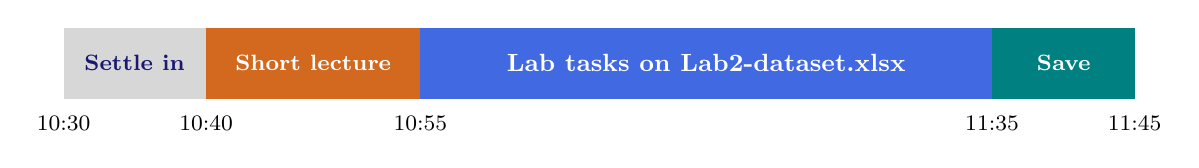
\begin{tikzpicture}[every node/.style={font=\small}]
 \fill[graytext!30]  (0,0)    rectangle (1.81,0.9);
 \fill[orangecustom] (1.81,0) rectangle (4.53,0.9);
 \fill[midblue]      (4.53,0) rectangle (11.79,0.9);
 \fill[tealcustom]   (11.79,0) rectangle (13.6,0.9);
 \node[text=darkblue] at (0.9,0.45) {\footnotesize\textbf{Settle in}};
 \node[text=white] at (3.17,0.45) {\footnotesize\textbf{Short lecture}};
 \node[text=white] at (8.16,0.45) {\textbf{Lab tasks on Lab2-dataset.xlsx}};
 \node[text=white] at (12.7,0.45) {\footnotesize\textbf{Save}};
 \node[anchor=north] at (0,-0.1) {\footnotesize 10:30};
 \node[anchor=north] at (1.81,-0.1) {\footnotesize 10:40};
 \node[anchor=north] at (4.53,-0.1) {\footnotesize 10:55};
 \node[anchor=north] at (11.79,-0.1) {\footnotesize 11:35};
 \node[anchor=north] at (13.6,-0.1) {\footnotesize 11:45};
\end{tikzpicture}
\end{center}

\vskip.12in
\begin{center}
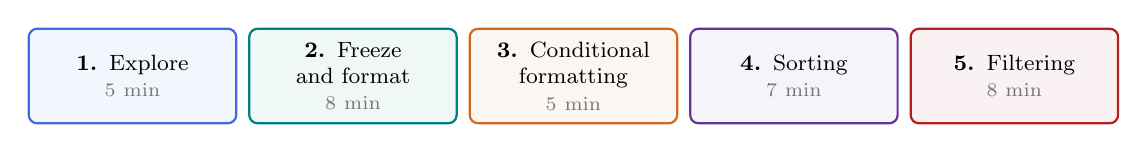
\begin{tikzpicture}[every node/.style={font=\footnotesize},
  t/.style={draw, rounded corners=3pt, thick, minimum width=2.55cm, minimum height=1.2cm, align=center, text width=2.4cm}]
 \node[t, draw=midblue, fill=midblue!6]           at (0,0)    {\textbf{1.} Explore\\\scriptsize\color{graytext}5 min};
 \node[t, draw=tealcustom, fill=tealcustom!6]     at (2.8,0)  {\textbf{2.} Freeze and format\\\scriptsize\color{graytext}8 min};
 \node[t, draw=orangecustom, fill=orangecustom!6] at (5.6,0)  {\textbf{3.} Conditional formatting\\\scriptsize\color{graytext}5 min};
 \node[t, draw=purplecustom, fill=purplecustom!6] at (8.4,0)  {\textbf{4.} Sorting\\\scriptsize\color{graytext}7 min};
 \node[t, draw=redcustom, fill=redcustom!6]       at (11.2,0) {\textbf{5.} Filtering\\\scriptsize\color{graytext}8 min};
\end{tikzpicture}
\end{center}

\vskip.12in
\begin{itemize}
\setlength{\itemsep}{0.5em}
\item {\color{purplecustom}Stuck?} Come back to the step-by-step slides in this lecture. They have every step
\item {\color{purplecustom}Save as} \texttt{RollNo\_Lab2.xlsx} and write your answers on the \textbf{Answers} sheet
\end{itemize}

\vskip.1in
\begin{block}{How the lab manual works}
\footnotesize
Each task tells you \textbf{what} to produce, not how to click. The how is on the step-by-step slides you just saw. Do the tasks in order, they get harder.
\end{block}
}

% %%%%%%%%%%%%%%%%%%%%%%%%%%%%%%%%%%%%%%%%%%%%%%%%%%%%%%%%%%%%
\section{Wrap-Up}
% %%%%%%%%%%%%%%%%%%%%%%%%%%%%%%%%%%%%%%%%%%%%%%%%%%%%%%%%%%%%

\frame[t]{\small
\vskip.0in
{\large{\color{blue}{\uline{Questions?\hfill}}}}
\vskip.12in

\begin{center}
\vskip.1in
{\Large\textcolor{purplecustom}{\textbf{Open Lab2-dataset.xlsx and start Task 1.}}}

\vskip.25in
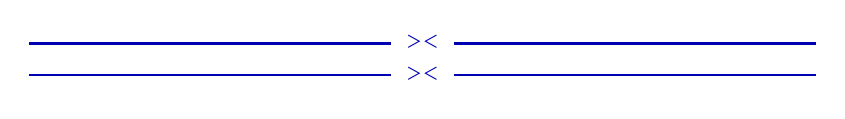
\begin{tikzpicture}
\draw[thick, blue!70!black] (-5,0) -- (-0.4,0);
\node[text=blue!70!black] at (0,0) {\texttt{><}};
\draw[thick, blue!70!black] (0.4,0) -- (5,0);
\draw[thick, blue!70!black] (-5,-0.4) -- (-0.4,-0.4);
\node[text=blue!70!black] at (0,-0.4) {\texttt{><}};
\draw[thick, blue!70!black] (0.4,-0.4) -- (5,-0.4);
\end{tikzpicture}

\vskip.12in
\textcolor{teal}{\small ICT 101: Applications of ICT Lab}

\vskip.2in
{\footnotesize\color{graytext}Try first, then ask. I will be walking around the lab.}
\end{center}
}

\end{document}
